\section{Бизнесийн үйл ажиллагааны шинжилгээ}
Бизнес процессийн модель нь чатбот системийн үндсэн процесс буюу үйл ажиллагааны явцыг BMPN-2.0 ашиглан дүрслэн харуулав \cite{BPMN}. Диаграммд дүрслэхдээ оролцогч талууд болох системүүдийг тус тусын \textit{pool} дотор дүрсэлсэн бол дэд процесс буюу \textit{subprocess}-ийг \textit{lane}-д дүрсэлж хоорондын хамаарлыг харууллаа. 
\begin{figure}[ht]
  \centering
  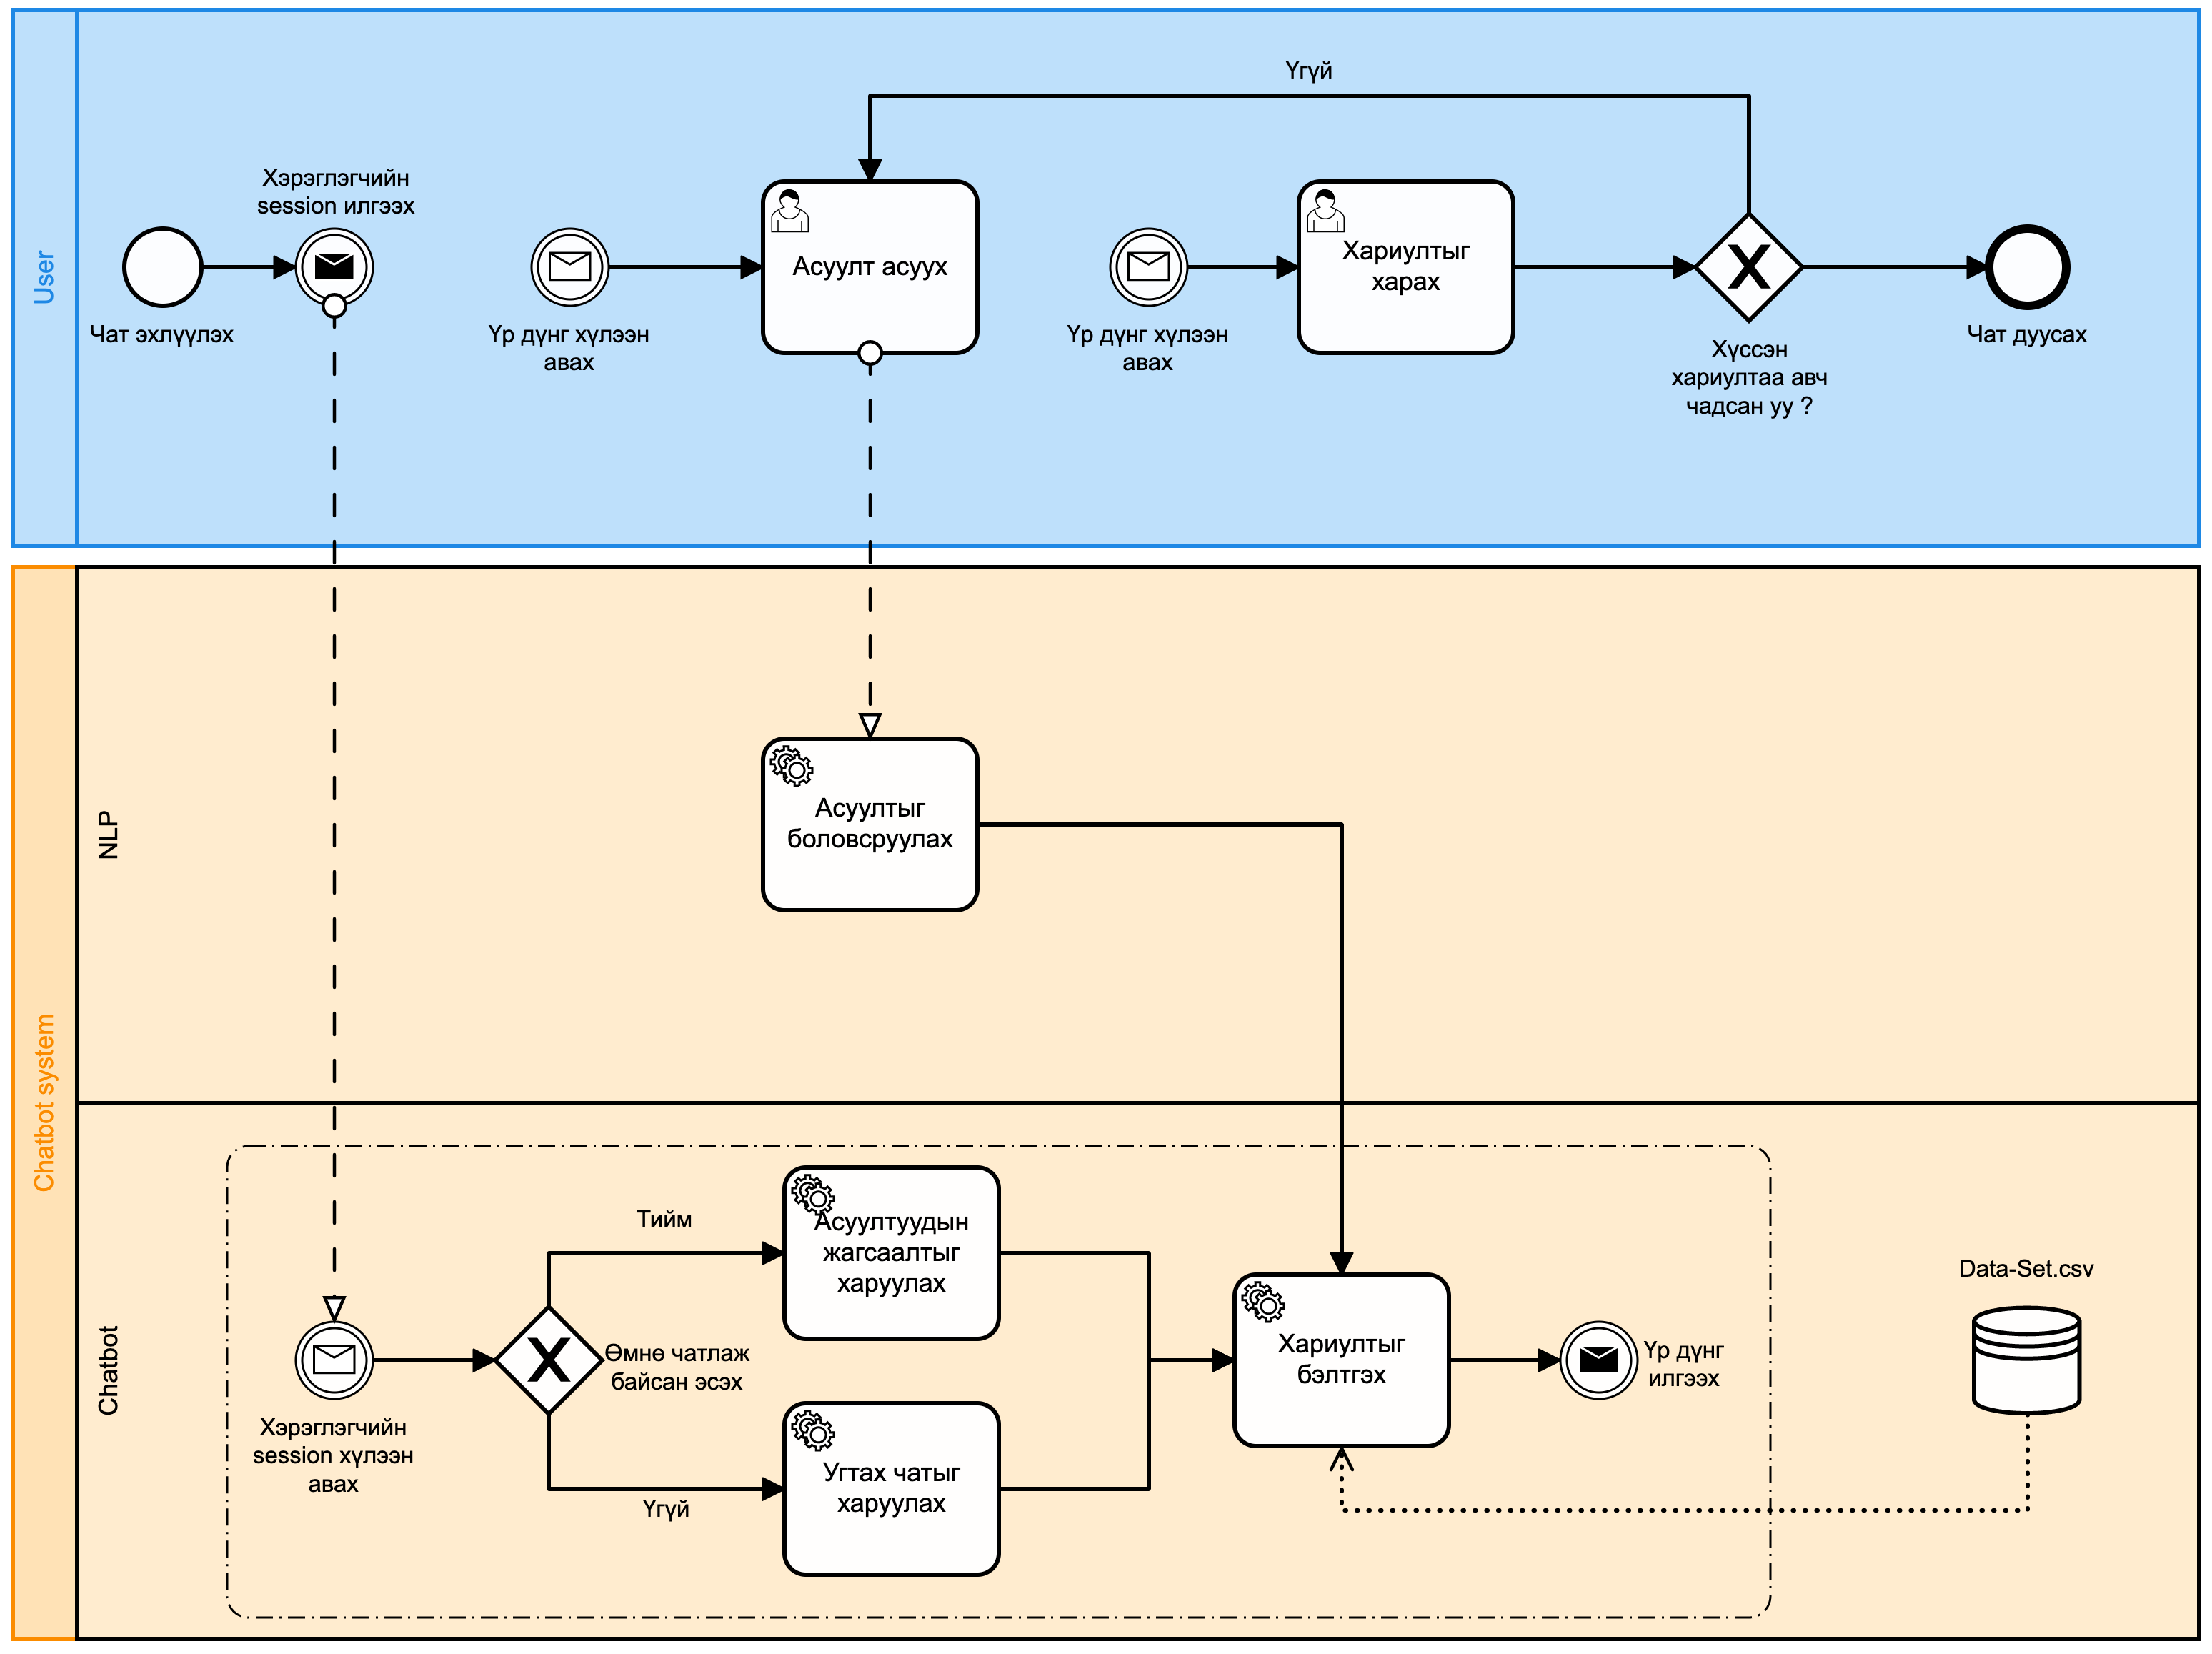
\includegraphics[width=\textwidth]{images/bpmn1.png}
  \caption{BPMN-1}\label{fig:bpmn1}
\end{figure}
\begin{figure}[ht]
\centering
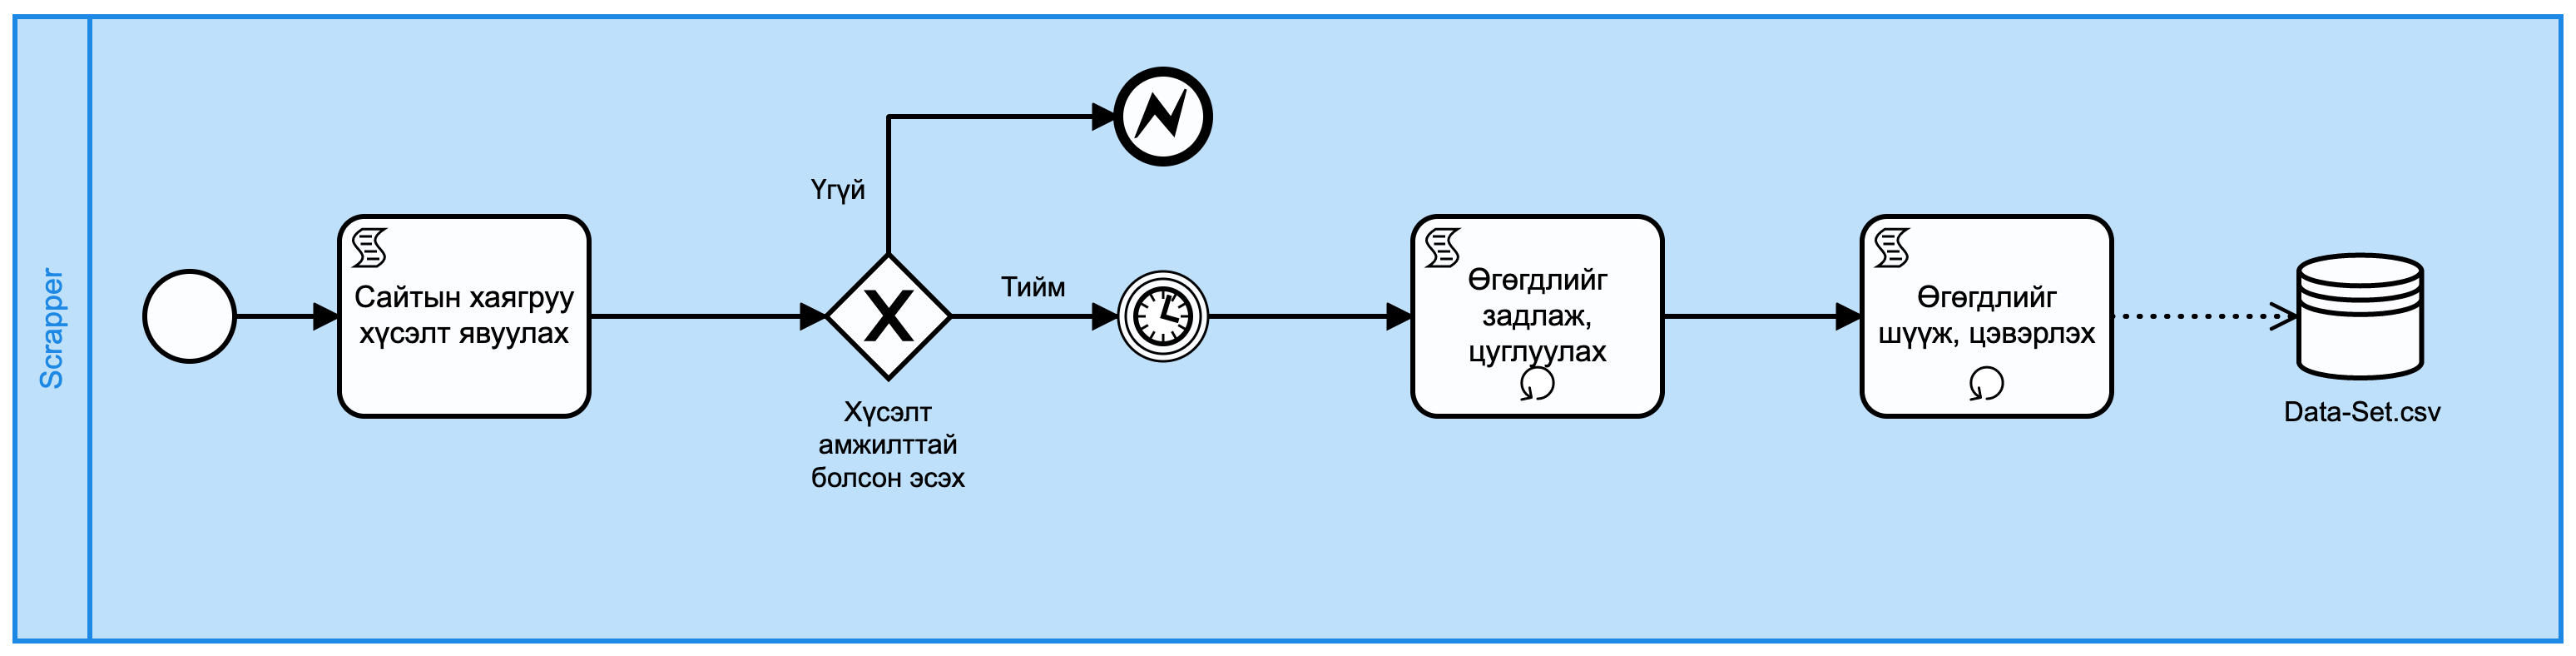
\includegraphics[width=\textwidth]{images/bpmn2.png}
\caption{BPMN-2}\label{fig:bpmn2}
\end{figure}
\section{Хэрэглэгч}
Чатбот системийг ямар ч хүн хэрэглэх боломжтой бөгөөд олон нийтэд нээлттэй байна. Системийн гол зорилго нь ажил хайж буй хэрэглэгчдэд ажлын байрны цогц мэдээллийг олгох зорилготой байх тул хэрэглэгчдийг дараах байдлаар тодорхойлж болно. Үүнд:
\begin{itemize}
  \item Ажлын байр хайж буй хүн
  \item Хөгжүүлэгч
\end{itemize}
\section{Функционал шаардлага}
Дараах хэсэгт чатбот системд тавигдах функционал шаардлагуудыг харуулсан болно.
\begin{itemize}
  \item[ФШ 1] Чатбот нь харилцан яриа эхэлмэгц хариу өгдөг байна. 
  \item[ФШ 2] Чатбот нь ямар ч оролтод хариу өгнө.
  \item[ФШ 3] Хэрэв чатбот нь оролтод хариу өгч чадхааргүй байвал бусад асуултуудыг санал болгож ойлгомжгүй утга оруулсныг илэрхийлнэ.
  \item[ФШ 4] Чатботын санал болгох асуултууд нь цэс хэлбэртэй харагдана.
  \item[ФШ 5] Чатботын цэсэн дээр нэг товшилтоор асуултын хариултыг харуулдаг байна.  
  \item[ФШ 6] Алхам бүрд үндсэн цэсрүү буцах сонголтыг харуулдаг байна. 
  \item[ФШ 7] Чатботны хариулт нь текстэн хэлбэрээр хэрэглэгчид харагдана.
  \item[ФШ 8] Чатбот нь зөвхөн Монголоор бичсэн асуултад хариулт өгнө.
  \item[ФШ 9] Чатбот нь дэлгэрэнгүй мэдээллийг цэс хэлбэрээр сонгуулан харуулж чаддаг байна. 
  
\end{itemize}
\section{Функционал бус шаардлага}
\quad\textbf{Бэлэн болон найдвартай байдал (Availability \& Reliability)}
\begin{itemize}
  \item[ФБШ 01] Чатбот систем өдрийн аль ч цагт 99.999\% ажиллагаатай байх ёстой.
  \item[ФБШ 02] Ямар ч хүсэлт ирсэн чатбот 100\% хариу өгдөг байна. 
\end{itemize}
\quad\quad\textbf{Гүйцэтгэлтэй байдал (Performance)}
\begin{itemize}
  \item[ФБШ 03] Чатботын байршуулсан сувагт, шаардлагаас хамаарч ямар ч төхөөрөмжөөс хандаж болно.
  \item[ФБШ 04] Зарим тохиолдолд чатботын гүйцэтгэл нь хэрэглэгчийн интернет болон төхөөрөмжийн үйлдлийн системийн хувилбараас хамаарч болно.
\end{itemize}
\quad\quad\textbf{Дэмжих чадвар (Supportability)}
\begin{itemize}
  \item[ФБШ 05] Чатботын эх кодыг \textit{github} дээр нээлттэй эхийн систем хэлбэрээр байршуулна.
\end{itemize}
\quad\quad\textbf{Хэрэгцээт байдал (Usability)}
\begin{itemize}
  \item[ФБШ 06] Чатбот нь хэрэглэхэд хялбар, ойлгомжтой байна.
  \item[ФБШ 07] Чатботны цэс нь ойлгомжтой цөөн үгээр илэрхийлэгдсэн байна. 
  \item[ФБШ 08] Чатботны цэсийн хэмжээ дарагдахуйц том байна.
\end{itemize}
\quad\quad\textbf{Аюулгүй байдал(Security)}
\begin{itemize}
  \item[ФБШ 09] Чатбот системийн байршуулсан сувгийн стандартын дагуу хэрэглэгчийн мэдээллийг өгөгдлийн санд хадгалахгүй байна.  
\end{itemize}
\section{Use case диаграмм}
Чатбот системийн use-case диаграммыг байдлаар тодорхойлов \cite{useCase}.
\begin{figure}[ht]
  \centering
  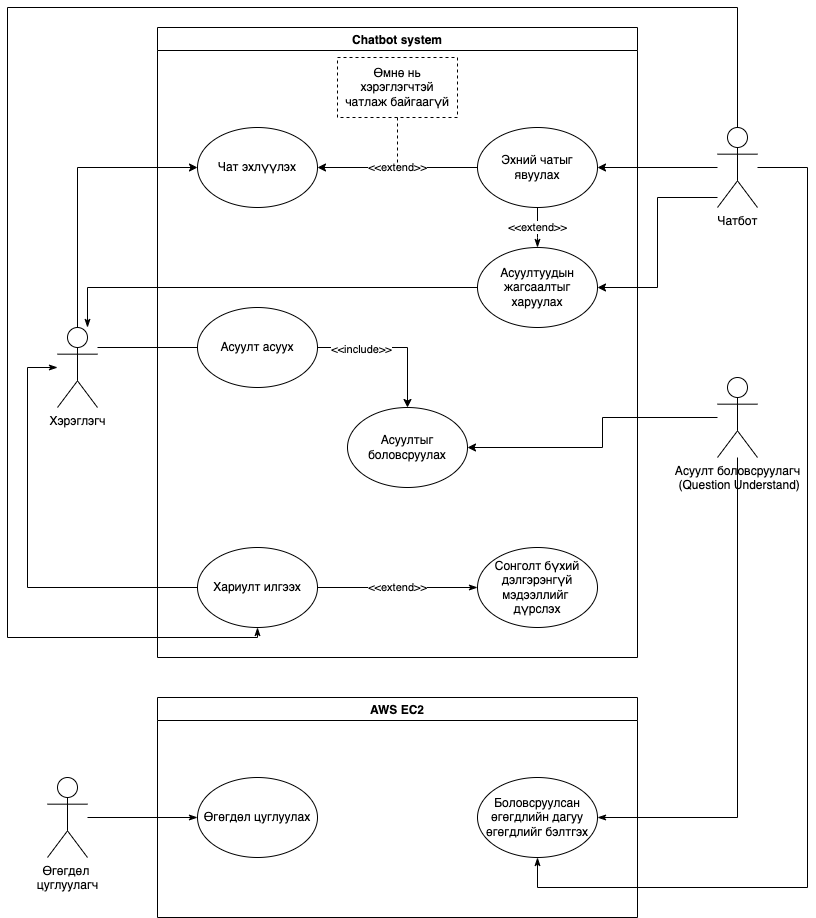
\includegraphics[width=\textwidth-2.2cm]{images/useCase.png}
  \caption{Use Case диаграмм}\label{fig:useCase}
\end{figure}
